% Multiple-choice exam only: four unmarked choices per question.
\noindent\begin{minipage}{\linewidth}
\small
\textbf{Câu 1.} Phát biểu nào mô tả đúng vai trò của workspace, compute và catalog trong Databricks?
\begin{enumerate}[label=\textbf{\Alph*.},leftmargin=2em,itemsep=0pt,topsep=2pt]
\item Workspace thực thi SQL; compute tổ chức bảng; catalog lưu notebook.
\item Workspace tổ chức bảng; compute lập lịch job; catalog cấp tài nguyên thực thi.
\item Workspace tổ chức công việc; compute thực thi câu lệnh; catalog tổ chức tài sản dữ liệu.
\item Workspace quản lý quyền bảng; compute lưu metadata; catalog thực thi notebook.
\end{enumerate}
\end{minipage}\par\addvspace{0.5em}

\noindent\begin{minipage}{\linewidth}
\small
\textbf{Câu 2.} Ngoài phân quyền truy cập, nhóm nội dung nào thuộc phạm vi data governance được giới thiệu trong bài?
\begin{enumerate}[label=\textbf{\Alph*.},leftmargin=2em,itemsep=0pt,topsep=2pt]
\item Tăng kích thước compute, mở thêm worker và tối ưu tốc độ CPU.
\item Quản lý metadata, xác định ownership, theo dõi lineage và xem xét audit log.
\item Đổi màu notebook, sắp xếp tab trình duyệt và lựa chọn giao diện.
\item Cài thư viện Python, viết biểu đồ và thay đổi phím tắt của trình soạn thảo.
\end{enumerate}
\end{minipage}\par\addvspace{0.5em}

\noindent\begin{minipage}{\linewidth}
\small
\textbf{Câu 3.} Tên bảng \texttt{lab\_governance.silver.orders\_clean} được hiểu đúng theo thứ tự nào?
\begin{enumerate}[label=\textbf{\Alph*.},leftmargin=2em,itemsep=0pt,topsep=2pt]
\item Catalog: orders\_clean; schema: silver; table: lab\_governance.
\item Catalog: silver; schema: lab\_governance; table: orders\_clean.
\item Catalog: lab\_governance; schema: orders\_clean; table: silver.
\item Catalog: lab\_governance; schema: silver; table: orders\_clean.
\end{enumerate}
\end{minipage}\par\addvspace{0.5em}

\noindent\begin{minipage}{\linewidth}
\small
\textbf{Câu 4.} Một user được sử dụng SQL warehouse nhưng chưa được cấp SELECT trên bảng cần đọc. Vì sao chưa thể kết luận user đọc được bảng?
\begin{enumerate}[label=\textbf{\Alph*.},leftmargin=2em,itemsep=0pt,topsep=2pt]
\item Quyền sử dụng compute và quyền truy cập dữ liệu thuộc các phạm vi khác nhau.
\item Quyền sử dụng warehouse tự động cấp SELECT cho mọi bảng.
\item Quyền SELECT chỉ được kiểm tra khi compute đang tắt.
\item Quyền bảng được xác định hoàn toàn bởi tên của warehouse.
\end{enumerate}
\end{minipage}\par\addvspace{0.5em}

\noindent\begin{minipage}{\linewidth}
\small
\textbf{Câu 5.} Một analyst đã có USE CATALOG và SELECT nhưng thiếu USE SCHEMA trên schema cha, kể cả qua nhóm hoặc kế thừa. Analyst có đủ quyền đọc bảng không?
\begin{enumerate}[label=\textbf{\Alph*.},leftmargin=2em,itemsep=0pt,topsep=2pt]
\item Có, vì SELECT là điều kiện duy nhất để đọc bảng.
\item Có, vì USE CATALOG luôn bao gồm USE SCHEMA.
\item Chưa; analyst cần có thêm USE SCHEMA trên schema cha.
\item Chưa; chỉ cần thêm MODIFY để thay thế USE SCHEMA.
\end{enumerate}
\end{minipage}\par\addvspace{0.5em}

\noindent\begin{minipage}{\linewidth}
\small
\textbf{Câu 6.} Giả sử đã có đủ quyền sử dụng namespace, SELECT cấp trên schema gold khác SELECT chỉ cấp trên bảng gold.daily\_sales như thế nào?
\begin{enumerate}[label=\textbf{\Alph*.},leftmargin=2em,itemsep=0pt,topsep=2pt]
\item Grant ở schema chỉ áp dụng cho bảng đã tồn tại tại thời điểm cấp quyền.
\item Grant ở schema có phạm vi rộng hơn, bao gồm các bảng phù hợp hiện có và tạo sau trong schema.
\item Grant ở schema chỉ cho xem metadata, không cho đọc dữ liệu.
\item Grant ở schema tự động cho phép UPDATE và DELETE trên các bảng.
\end{enumerate}
\end{minipage}\par\addvspace{0.5em}

\Needspace{16\baselineskip}
\section*{Vận dụng: phân tích tình huống}
\noindent\begin{minipage}{\linewidth}
\small
\textbf{Câu 7.} Mai đọc được bảng silver khi chạy notebook bằng tài khoản cá nhân. Khi Mai kích hoạt job, kết quả từng task và danh tính chạy được ghi trong sơ đồ.
\par\smallskip
\noindent\makebox[\linewidth][c]{
\includegraphics[width=0.96\linewidth]{Figures/case-7.png}}\par\smallskip
Thay đổi nhỏ nhất để sửa đúng lỗi mà vẫn giữ danh tính vận hành là gì?
\begin{enumerate}[label=\textbf{\Alph*.},leftmargin=2em,itemsep=0pt,topsep=2pt]
\item Cấp SELECT trên \texttt{silver.orders\_clean} cho \texttt{sp\_sales} rồi chạy lại task bị lỗi.
\item Cấp thêm SELECT trên \texttt{silver.orders\_clean} cho Mai vì Mai là người bấm chạy.
\item Đổi Run as sang Mai để quyền của job luôn đi theo người đang vận hành.
\item Cấp SELECT ở cấp catalog cho \texttt{sp\_sales} để job có thể đọc cả các bảng sẽ tạo sau này.
\end{enumerate}
\end{minipage}\par\addvspace{0.5em}

\noindent\begin{minipage}{\linewidth}
\small
\textbf{Câu 8.} Sơ đồ mô tả thao tác của job và bảng duy nhất analyst cần đọc.
\par\smallskip
\noindent\makebox[\linewidth][c]{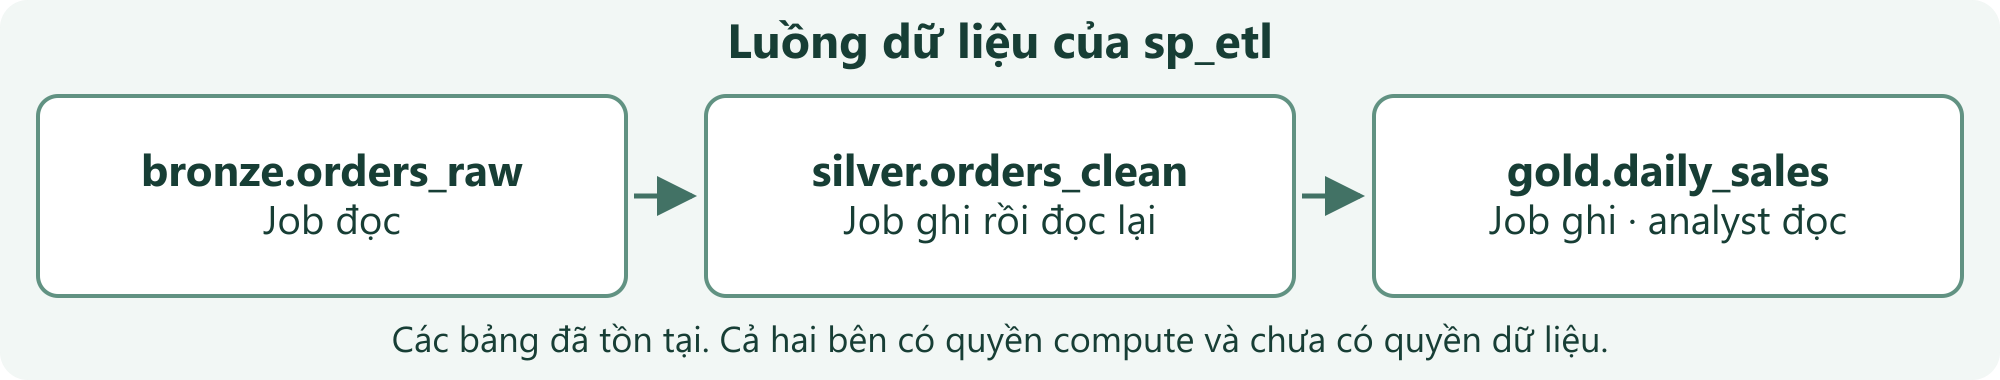
\includegraphics[width=0.96\linewidth]{Figures/case-8.png}}\par\smallskip
Phương án nào đáp ứng cả hai luồng công việc và giữ phạm vi quyền hẹp?
\begin{enumerate}[label=\textbf{\Alph*.},leftmargin=2em,itemsep=0pt,topsep=2pt]
\item Cấp SELECT toàn catalog cho cả hai bên, rồi cấp MODIFY ở gold cho \texttt{sp\_etl}.
\item Cấp \texttt{sp\_etl} quyền đọc bronze, đọc/ghi silver, ghi gold trên từng bảng; cấp analyst quyền sử dụng catalog, schema gold và SELECT đúng bảng báo cáo; cấp \texttt{sp\_etl} quyền sử dụng các namespace cần thiết.
\item Cấp quyền tạo bảng ở silver và gold cho \texttt{sp\_etl}; cấp analyst SELECT trên bảng gold mà không cấp quyền sử dụng schema.
\item Cho analyst đọc bảng silver thay cho gold; dùng quyền chạy job để \texttt{sp\_etl} tự đọc và ghi các bảng.
\end{enumerate}
\end{minipage}\par\addvspace{0.5em}

\noindent\begin{minipage}{\linewidth}
\small
\textbf{Câu 9.} Nhóm cần xác định bước nào làm sai số liệu và danh tính nào thực hiện thao tác liên quan quanh thời điểm đó.
\par\smallskip
\noindent\makebox[\linewidth][c]{
\includegraphics[width=0.96\linewidth]{Figures/case-9.png}}\par\smallskip
Thứ tự điều tra nào có khả năng phân biệt lỗi biến đổi với thay đổi dữ liệu ngoài dự kiến?
\begin{enumerate}[label=\textbf{\Alph*.},leftmargin=2em,itemsep=0pt,topsep=2pt]
\item Dùng audit log để tự suy ra công thức tổng hợp rồi sửa dashboard ngay.
\item Xem trạng thái job thành công và chỉ kiểm tra cấu hình SQL warehouse.
\item Chỉ đọc lineage; nếu thấy đủ ba tầng thì kết luận không có lỗi ở pipeline.
\item Dùng lineage xác định nguồn và task liên quan; đối chiếu số dòng, số đơn duy nhất và phép tổng hợp theo từng tầng; xem audit để xác định hoạt động và danh tính trong khoảng thời gian đó.
\end{enumerate}
\end{minipage}\par\addvspace{0.5em}

\noindent\begin{minipage}{\linewidth}
\small
\textbf{Câu 10.} Lan vẫn đọc được bảng chi tiết. Sau thay đổi, analyst phải còn đọc được daily\_sales và job vẫn cần ghi cả hai bảng.
\par\smallskip
\noindent\makebox[\linewidth][c]{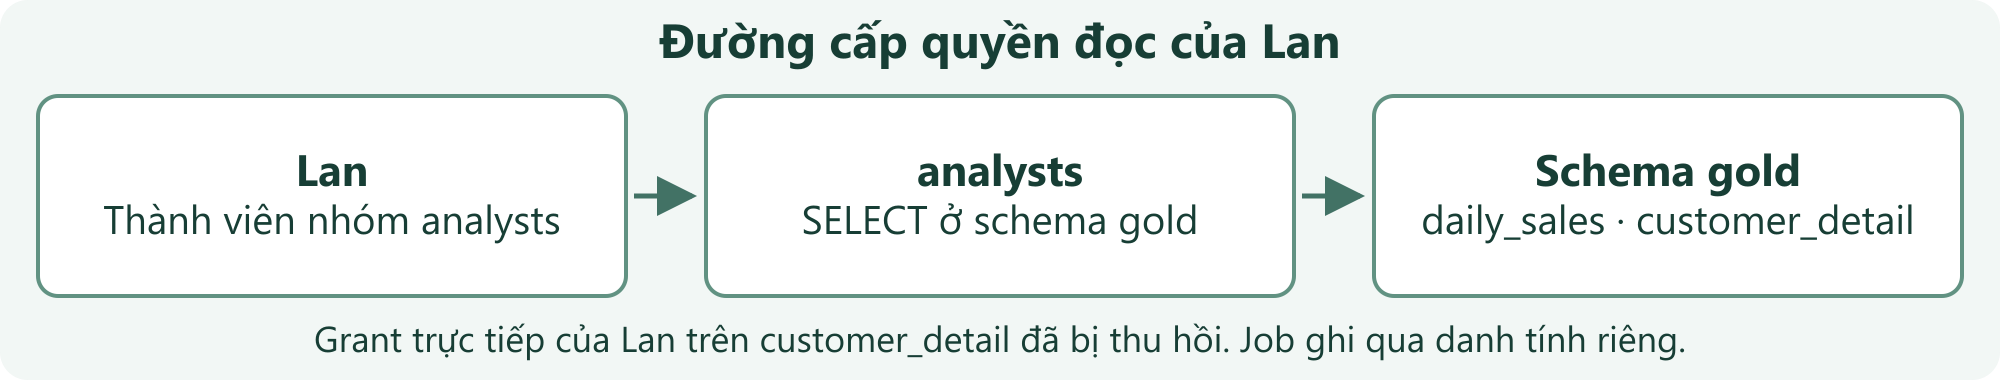
\includegraphics[width=0.96\linewidth]{Figures/case-10.png}}\par\smallskip
Kế hoạch nào đúng với mục tiêu?
\begin{enumerate}[label=\textbf{\Alph*.},leftmargin=2em,itemsep=0pt,topsep=2pt]
\item Thu hồi USE SCHEMA gold của analyst để chặn bảng chi tiết; giữ nguyên các grant SELECT hiện tại.
\item Chạy thử bằng owner; nếu owner đọc được cả hai bảng thì quyền analyst đã đúng.
\item Cấp SELECT riêng trên \texttt{daily\_sales} cho \texttt{analysts}, gỡ SELECT ở schema và rà các grant khác; thử lại bằng tài khoản analyst và xác nhận job vẫn chạy bằng danh tính riêng.
\item Gỡ quyền ghi của service principal trên \texttt{customer\_detail} để ngăn Lan đọc bảng.
\end{enumerate}
\end{minipage}\par\addvspace{0.5em}
